\section{Simulation}
\subsection{Kontinuer controller}
For at teste den kontinuere controller's respons modelleres systemet ud fra state space repræsentationen og de fundne K-værdier til følgende blokdiagram \autoref{fig:Simulink_blokdiagram_1}, uden brug af observer i første omgang. 

\begin{figure}[H]
	\centering
	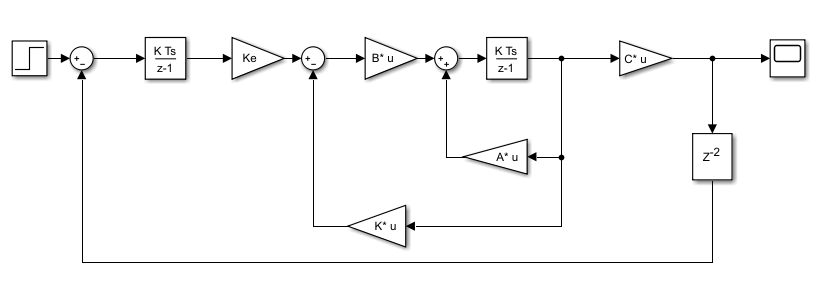
\includegraphics[width = 1\textwidth]{figur/Simulink_blokdiagram_1}
	\caption{Blok diagram for den kontinuere controller uden observer}
	\label{fig:Simulink_blokdiagram_1}
\end{figure}

State matricen hentes direkte fra modellen ligesom i Matlab. Delay blokken med 2 unit delay skyldes, at gerne vi simulere at gyroskopet på udgangen bruger 1 delay på at sample og 1 delay på at integrere den samplede vinkelhastighed til en vinkel. Ved at sende et step med amplituden 30 ind som reference signal forventer vi derfor, at kunne måle en værdi på 30 på outputtet efter cirka halvt sekund efter steppet. Dette kan ses i scopet i \autoref{fig:Simulink_scope_1}.

\begin{figure}[H]
	\centering
	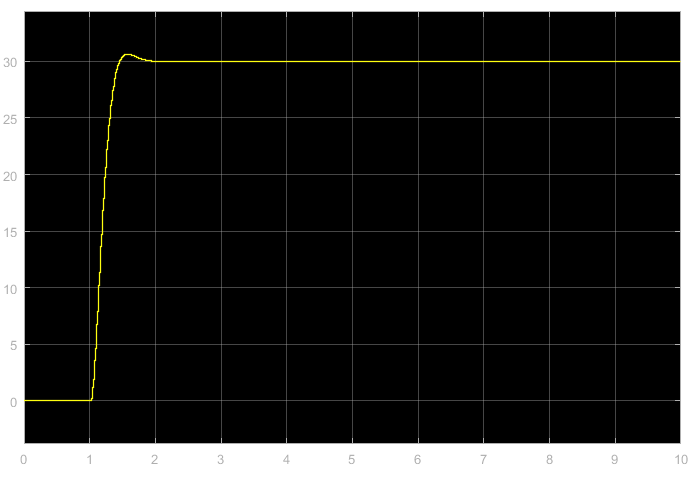
\includegraphics[width = 0.75\textwidth]{figur/Simulink_scope_1}
	\caption{Step respons (Amplitude = 30) for den kontinuere controller uden observer}
	\label{fig:Simulink_scope_1}
\end{figure}

Resultatet i \autoref{fig:Simulink_scope_1} passer med forventningerne med settling time og ingen steady state error. Dog ses der et lille overshoot på cirka 1.5\%, hvilket tyder på at systemet er blevet lidt mindre stabilt pga delay blokken med 2 unit delay. Dette har dog minimal betydning, da kravet om max 5\% overhoot stadig overholdes.

Men som nævnt tidligere kan man ikke hente state matricen direkte ud fra systemet, så derfor tilføjes en observer til blokdiagrammet i \autoref{fig:Simulink_blokdiagram_1} så state matrixen kan hentes fra outputtet i stedet. Dette kan ses herunder i \autoref{fig:Simulink_blokdiagram_2}.

\begin{figure}[H]
	\centering
	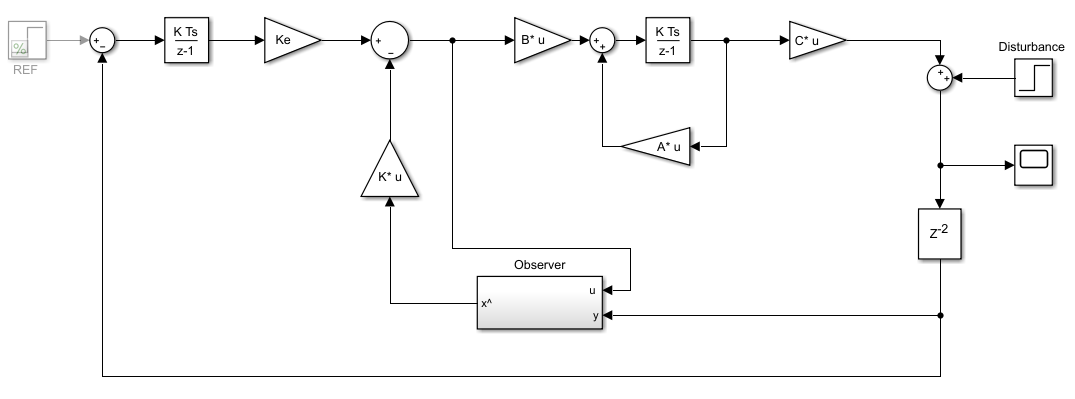
\includegraphics[width = 1\textwidth]{figur/Simulink_blokdiagram_2}
	\caption{Blok diagram for den kontinuere controller med observer}
	\label{fig:Simulink_blokdiagram_2}
\end{figure}
I \autoref{fig:Simulink_blokdiagram_2} ses det at observeren har outputtet fra gyroskoppet som input sammen med inputtet til motorblokken (state space repræsentation) og spytter states matricen ud, som føres tilbage med forstærkningensmatricen K . Observeren er implementeret ud fra det tidligere design og kan ses i \autoref{fig:Simulink_observer_continues}. Ved at sende et step med amplituden 30 ind som forstyrrelse signal på outputtet (forstyrrelse fra overfladens hælding) forventer vi derfor, at kunne måle en værdi på 0 på outputtet efter cirka halvt sekund efter steppet, hvis referencesignalet sættes til 0. Dette kan ses i scopet i \autoref{fig:Simulink_scope_2}.
 
\begin{figure}[H]
	\centering
	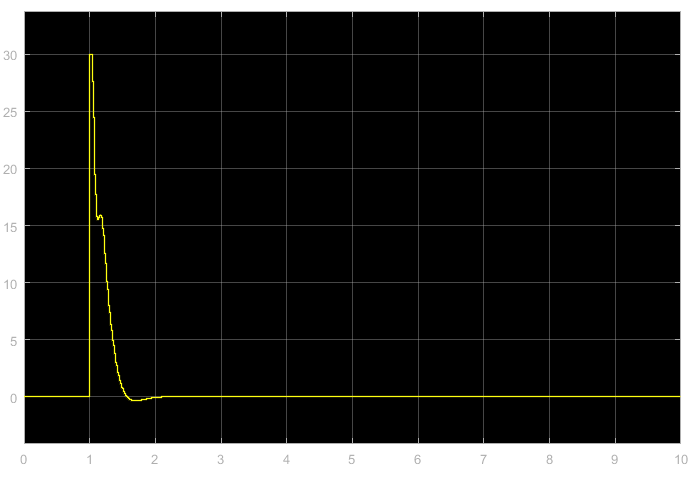
\includegraphics[width = 0.75\textwidth]{figur/Simulink_scope_2}
	\caption{Step respons for den kontinuere controller med observer påsat forstyrrelse på outputtet (Amplitude = 30)}
	\label{fig:Simulink_scope_2}
\end{figure}

Resultatet i \autoref{fig:Simulink_scope_2} passer med forventningerne og viser at systemet regulere tilbage til vandret efter cirka et halvt sekund, hvis det bliver udsat for en forstyrrelse. Dog ses det at, reguleringen ikke sker helt jævnt, hvilket formentlig skyldes at observeren påvirker systemet med sine poler og ikke gætter 100\% rigtig på state matricen, hvormed resultatet påvirkes. Dette er dog acceptabelt, idet systemet stadig finder tilbage på plads uden alt for meget oscillation. 

\subsection{Diskret controller}
For at teste den ufuldstændige diskrete controller's respons modelleres systemet ud fra state space repræsentationen og de fundne Kd-værdier til følgende blokdiagram \autoref{fig:Simulink_blokdiagram_3}, uden brug af observer i første omgang. 

\begin{figure}[H]
	\centering
	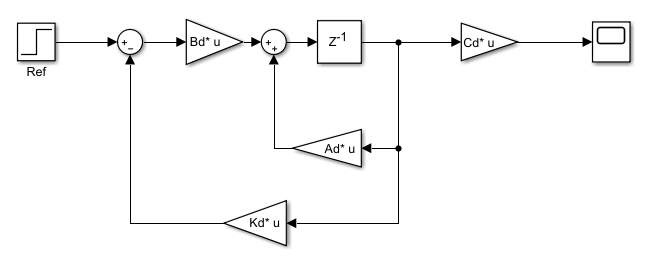
\includegraphics[width = 0.80\textwidth]{figur/Simulink_blokdiagram_3}
	\caption{Blok diagram for den diskrete controller uden observer og uden korrektion for steady state error}
	\label{fig:Simulink_blokdiagram_3}
\end{figure}

State matricen hentes direkte fra modellen ligesom i Matlab. Det er værd at bemærke, at hvor der før i den kontinuere state space model var et integrationsblok er denne ny byttet ud med en unit delay blok for at realisere den samplede state matrix. Ved at sende et step med amplituden 30 ind som reference signal forventer vi, at systemet falder til efter cirka halvt sekund efter steppet og ikke har noget betydeligt overshoot. Dette kan ses i scopet i \autoref{fig:Simulink_scope_3}.

\begin{figure}[H]
	\centering
	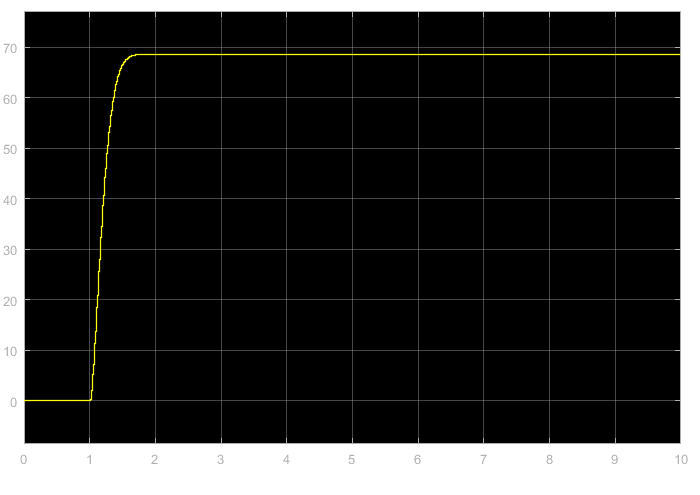
\includegraphics[width = 0.75\textwidth]{figur/Simulink_scope_3}
	\caption{Step respons (Amplitude = 30) for diskrete controller uden observer og uden korrektion for steady state error}
	\label{fig:Simulink_scope_3}
\end{figure}

Resultatet i \autoref{fig:Simulink_scope_1} passer med forventningerne med settling time og overshoot. Den stationære værdi er for høj, hvilket skyldes at denne controller ikke har nogen korrektion for steady state error med et integrationsled i loopet ligesom den kontinuere controller. Igen kan man ikke i praksis hente state matricen direkte ud fra systemet som her, så derfor tilføjes en observer til blokdiagrammet i \autoref{fig:Simulink_blokdiagram_3}, så state matrixen kan hentes fra outputtet i stedet. Dette kan ses herunder i \autoref{fig:Simulink_blokdiagram_4}.

\begin{figure}[H]
	\centering
	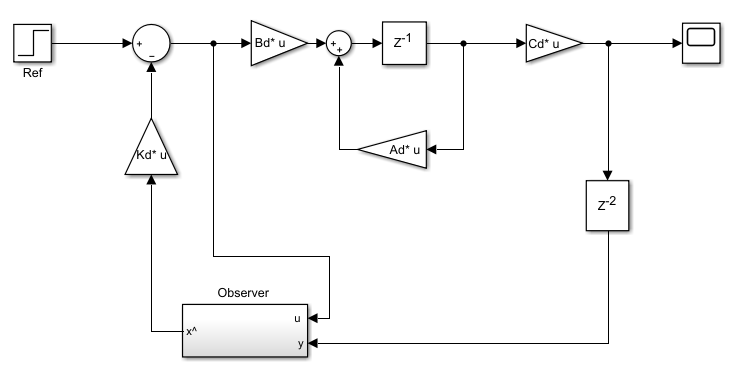
\includegraphics[width = 0.8\textwidth]{figur/Simulink_blokdiagram_4}
	\caption{Blok diagram for den diskrete controller med observer og uden korrektion for steady state error}
	\label{fig:Simulink_blokdiagram_4}
\end{figure}

I \autoref{fig:Simulink_blokdiagram_4} ses det, at observeren har outputtet fra gyroskoppet som input sammen med inputtet til motorblokken (state space repræsentation) og spytter states matricen ud, som føres tilbage med forstærkningensmatricen Kd. Observeren er implementeret ud fra det tidligere design og kan ses i \autoref{fig:Simulink_observer_diskret}. Ved igen at sende et step med amplituden 30 ind som reference signal, forventer vi at systemet falder til efter cirka halvt sekund efter steppet og ikke har noget betydeligt overshoot, præcis ligesom før uden observer. Dette kan ses i scopet i \autoref{fig:Simulink_scope_4}.

\begin{figure}[H]
	\centering
	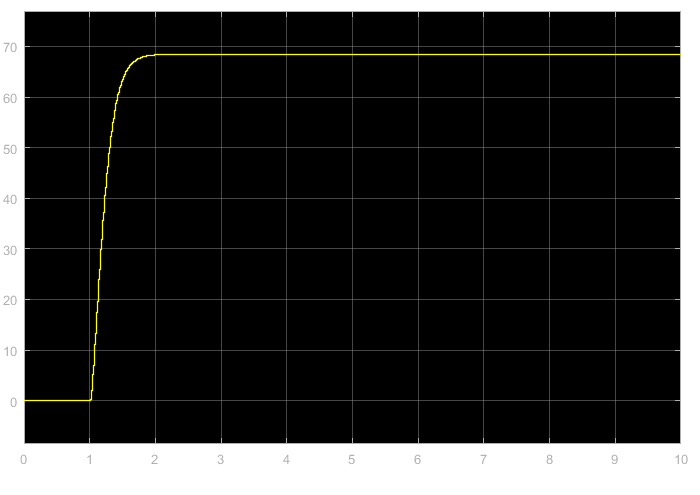
\includegraphics[width = 0.75\textwidth]{figur/Simulink_scope_4}
	\caption{Step respons (Amplitude = 30) for diskrete controller med observer og uden korrektion for steady state error}
	\label{fig:Simulink_scope_4}
\end{figure}

Resultatet i \autoref{fig:Simulink_scope_4} viser det samme som i \autoref{fig:Simulink_scope_3}, hvormed det kan konkluderes at observeren virker som forventet. Den eneste forskel er, at systemet virker en anelse langsommere, formentlig fordi observeren ikke gætter 100\% rigtig på state matricen, hvormed resultatet påvirkes.
 




